\documentclass{article}
\usepackage[french]{babel}
\usepackage[T1]{fontenc}
\usepackage[utf8]{inputenc}
\usepackage{graphicx}
\usepackage{eurosym}
\usepackage {times}
\usepackage{fancyhdr}
\usepackage{bm}
\usepackage{listings}
\title{Projet CamlT'OCR par SMK \\ Cahier des charges}
\pagestyle{fancyplain} \lhead{\textit{Projet CamelT'OCR}} \rhead{\textit{SMK}}
\date{24-10-2014}
\author{
    Timothe \textit{Tim-Tim} Bureau-Godart(bureau\_t) \and
        Leopold \textit{Meta} Szabatura (szabat\_l) \and
        Louis \textit{Zab} Forget (forget\_l) \and
        Maxime \textit{Kylox} Gaudron (gaudro\_m)
        1      }


\begin{document}
\maketitle
\tableofcontents
\newpage
\section{Introduction}
\addcontentsline{toc}{section}{Introduction}
Dans le cadre de notre spécialisation en informatique à l'EPITA, nous avons eu comme projet semestrielle la realisation d'un ocr ( Optical Character Recognition). Ce projet ce déroule sur 4 mois en Ocaml, un langage devellopé par l'INRIA. Nous présentons donc dans ce rapport l'état d'avancement du projet à la vielle de la premiere soutenance. Ce projet a été réalise par quatre membres fideles et dévoués à la bonne cause celle de notre ocr ! 
\subsection{presentation des membres}
\subsubsection{Louis "\textit{Zab}" Forget}
J'ai toujours etais tres curieux, au point de partir souvent dans tous les sens. J'ai toujours voulu savoir comment marchent les pages webs. C'est dans cette optique que j'ai appris a faire du HTML et CSS en troisieme. J'ai ensuite voulu savoir comment marchent les jeux videos, puis divers programmes. Il y a quelques jours je me suis demandais commemt marchent les gps qui indiquent la densite du traffic.
\subsubsection{Timothe "\textit{Tim-Tim}" Bureau Godart}
Je n'étais encore qu'un gosse quand le drame s'est produit, une attaque de livre dans ma propre maison ! J'étais dépassé, tous ses mots sans définition, tous ses paragraphes sans résumé, j'allais sombrer dans un univers d'horreur et d'épouvante sans pouvoir en ressortir... Quand soudain, la lumière apparu, elle avait la forme d'une gameboy géante et me sauva de l'enfer des livres. Depuis ce jour je lui voue un culte sans précédent et cherche à percer tous ses mystères.
Très jeune, je possédais déjà mon propre ordinateur, construis par un ami de mes parent, dès lors je n'ai jamais acheté d'ordinateur, je les ai toujours eu en pièce détaché. Cependant je ne m'intéressais pas trop a la programmation bien que cela me titillais un peu de ne pas savoir comment mes personnages de jeux vidéo pouvais attaquer sur la simple pression d'un bouton (car oui, je suis un grand fan de jeu vidéo et j'ai commencé très petit, ce qui est vite devenu une grande passion). J'ai commencé a réellement m'intéresser à cette univers en classe de seconde, grâce à l'option MPI. Je me suis documenté sur plusieurs langages quand j'ai entendu parler d'EPITA, ce qui m'a donné un but, faire partie de cette école pour faire de ma passion mon métier.
\subsubsection{Leopold "\textit{Meta}" Szabatura}
Je me suis intéressé à l'informatique à l’âge de 15 ans.
C'est pendant cette année de seconde que, en fouillant sur ma calculatrice, j'ai découvert l'univers fantastique de la programmation.
Cela m'a rapidement mené sur la voix du java ou je faisais mes premiers pas dans le monde de la programmation oriente objet.
\subsubsection{Maxime "\textit{kylox}" Gaudron}
J'ai toujours vécu dans un monde plus ou moin informatisé. Adepte de tout les petits appareils electroniques et mecaniques. A tel point que je démontais tout et que plus rien ne marchait ! Je me suis donc mis naturellement à aller chercher un peu plus loin dans le fonctionement interne des appareils. L'ocr est donc pour moi un grand apprentissage et une decouverte qui permet d'envisager differente possibilite de reconnaissance et de systemes automatisé ! 
\subsection{organisation du projet}
\newpage
\section{Les taches}
\subsection{quelque mots sur le site internet}
Pour commencer, vous pouvez trouver notre site web à l'adresse suivante : cmalt-ocr.epiproject.eu.\\
Pour ce site, nous avons décidé de commencer avec une interface simple, épuré et pas très rechercher pour facilité la navigation. Pour cela, nous n'avons utilisé que du HTML et du CSS. Cependant, nous ne comptons pas en rester la, nous envisageons de le continuer et de l'améliorer au file du temps, ainsi nous pourrons avoir un site beau et esthétique pour la dernière soutenance.\\ 
\subsection{Interface graphique}
Ce projet est pour nous le moyen de découvrir les bases et les approffondissements de la programmation d’un OCR, et d’en avoir (dans cette partie) une première approche simple et concrète de l’interface graphique. Pour une première approche, nous avons décidé de vous présenter une interface fonctionnelle, afin de vous donner une vision simpliste d’un OCR achevé. Pour cela, nous avons utilisé la lablGTK, qui est est un éditeur d’interface plutôt intuitif se basant sur un principe simple : pour créer une interface, on commence par créer une fenetre dans laquelle on met des «boites» qui vont contenir ce que l’on appelle des widgets (ou gadgets en français). Ces derniers peuvent servir à diffentes choses, du genre mettre une image ou encore des boutons.\\
L’interface graphique est un composant important pour notre projet puisqu’elle sera le seul contact qu’aura l’utilisateur avec notre programme. Par conséquent, cette dernière  devra être claire, simple d’utilisation et un minimum attractive pour l’utilisateur.\\
Cette interface graphique constitue mine de rien un enjeu assez important, étant
donné que c’est elle qui va permettre à l’utilisateur d’avoir accès à toutes les fonctionnalités. Elle se doit donc d’être intuitive et très simple d’utilisation et, dès son premier abord, l’utilisateur doit se sentir à l’aise avec chaque fonctionnalité pour apprécier le logiciel.

\subsubsection{Les box}
Ces derniers représentent la logique de Gtk, ce sont les éléments principaux
de l’interface graphique au niveau de sa conception car ils ne sont pas vraiment
visible une fois cette dernière terminée. Néanmoins cette logique a ses limites
car l’imbrication d’éléments les uns dans les autres nécessite beaucoup d’appels
et de très bien penser son interface avant même de l’avoir commencé.
Ces éléments primordiaux dans le travail de l’interface se décomposent en
deux sous-catégories, les hbox et les vbox. Les premières permettent d’empiler
les éléments de manière horizontale et les secondes servent à les empiler
de manière verticales. Une troisième catégorie un peu plus spécifique existe, il
s’agit des Gtktables, ces dernières permettent de créer des box dans un tableau
dont on peut déterminer la largeur et la hauteur et ainsi de créer une interface
un peu plus équilibrée.
Une fois la logique de ces éléments comprise, le travail consiste surtout à
savoir où placer les éléments et à déterminer leurs actions dans l’interface.

\subsubsection{Les widgets}
Ces éléments constituent le coeur graphique de l’interface. Il existe différents types de widgets, ceux destinés à afficher quelque chose comme une image ou du texte, ceux censés déterminer une action immédiate tels les boutons (contenant généralement une icône) et ceux contenant d’autres widgets à actions
immédiates tels que les barres d’outils.



\subsection{Traitement d'image}
\subsubsection{Le niveau de gris}
\subsubsubsection{\textbf{Le concept}}:\\
Une image se compose d'élément appelé pixel et definie par trois composante (en realite quattres mais ceci est une autre histoire) qui sont R,G et B correspondant au valeur Red, Green et Blue d'un pixel. Cette etape est primordiale car elle va permettre le bon traitement de l'image par l'ensemble des étapes aui la succède.\\
\subsubsubsection{\textbf{La realisation}}:\\
Pour réaliser ce niveau de gris on va travailler sur les trois composantes d'un pixel et appliquer la fromule suivante :
\\
\begin{center}
\[x = \frac{0.299 \times R + 0.587 \times G + 0.114 \times B}{3}\]
\end{center}
à l'ensemble des pixels de l'image. Le niveau de gris est operationel dans notre ocr, nous pouvons donc passer à la tache suivante.
\begin{figure}[h]
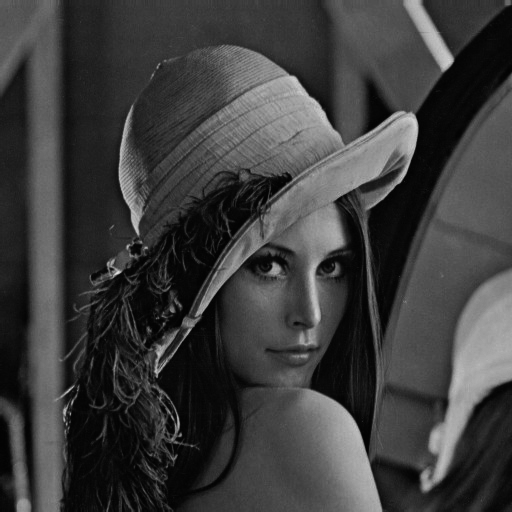
\includegraphics[width=0.50\textwidth]{img/grey.png}
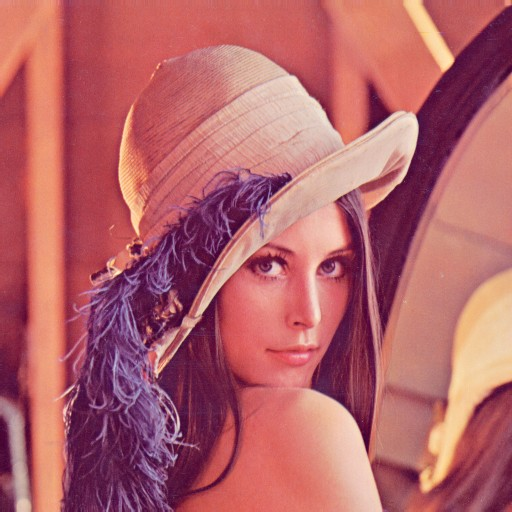
\includegraphics[width=0.50\textwidth]{img/lena.jpg}
\caption{avec et sans nuance (captain obvious is obvious)}
\end{figure}
\newpage{}
\subsubsection{Le filtre median}
\textbf{Le concept}:\\
Le filtre median va pour chaque pixels de l'image recuperer le triplet (R,G,B) de chaque pixel autour du pixel traitré et trier ces pixels par ordre croissant. Il suffit juste de recuperer la valeur mediane de la liste trier. Le passe dans cette algo et qyue l'on doit passer les pixels sur une autre image pour pas fausser les calculs sur la premiere image !
\vspace{0.8cm}
\textbf{La realisation}:\\
En pratique ce filtre ne s'applique pas sur toute les images car sinon elle floute l'image et la rend intraitable. Je suis actuellement en recherche d'un algorithme permettant de palier ce gros probleme. Au niveau aulgoritemiaue on obtiens
\vspace{0.8cm}
\begin{figure}[h]
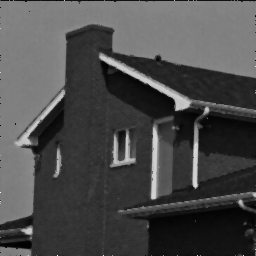
\includegraphics[width=0.50\textwidth]{img/house.png}
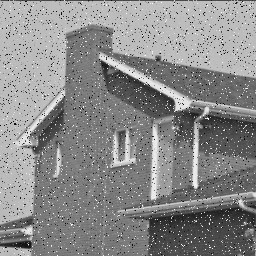
\includegraphics[width=0.50\textwidth]{img/house.jpg}
\caption{presentation du filtre median}
\end{figure}
\newpage
\subsubsection{La binarisation}
\subsubsubsection{\textbef{Le concept}}:\\
Nous utilisons l'algorithme d'Otsu, du nom de son inventeur Nobuyuki Otsu. Qui se base sur l'histogramme d'un image. L'histogramme est un tableau de 255 element, ici des entiers, qui represente le nombre d'occurence d'un niveau de gris ( les niveau de gris allant de 0 (blanc) a 255 (noir). Dans un permier temps va creer un tableau pour y mettre les valeur traiter de l'histogramme de la maniere suivante 
\begin{center}
\[ p_{i} = \frac{h_{i}} {width * height}\]
\end{center}
qui renvoie la population du niveau de gris i dans l'ensemble des pixels de l'image.
Nous allons ensuite traiter tout les pixels de l'image en fonction de ce tableau et de deux autres formules magique ! qui sont pour un pixel k :\\
\begin{minipage}[h]{5cm}
\begin{lstlisting}
v = 0;
for i = 0 to k do 
  v = v + h.(i) * i 
done
return v
\end{lstlisting}
\end{minipage}
\begin{minipage}[h]{5cm}
\begin{lstlisting}
m = 0
for i = 0 to k do
  m = m +. h.(i) * i
done 
return m
\end{lstlisting}
\end{minipage}
\vspace{0.8cm}
\\Le tout est injecter dans la formule

\[ s = v(i,p) \times (1 - v(i,p) \times (p.(255)) \times v(i,p) - m(i,p))^{2}\]
 
\subsubsection{Détection d'angle}
Je me suis donc occupe de la transformation de Hough. La transforme de hough est une techmiaue de reconnaissance de formes invente en 1962 par Paul Hough.
Le principe qui sous-tend la transforme de Hough est qu'il existe un nombre infini de ligne passant par un point dont la seule difference est l'orientation (l'angle). La transforme generalise de Houg fonctionne sur le principe qu'une droite peux s'ecrire sous la forme 
\[r = x\cos{\theta}+y\sin{\theta}\]
A chaque pixels noir on essaye de trouver la vlauer maximum de r. Cette valeur represente la droite qui alligne le plus de pixel noir. On la retiens et on vote dans un tableau pour son angle associer. On recommence sur tout les pixels. L'angle qui a recu le plus de vote estl'anlge de rotation de l'image( minore de la moitier de l'intervalle pour pouvoir faire ressortir les angles negatifs).
\\
Voici le principe de l'algo en pseudo code :
\begin{lstlisting}
for y =0 to hauteur de l'image do
    for x =0 to largeur de l'image do
        if (pixel noir ) then
           angle = -Pi/2
           while (angle < Pi/2) do
            begin
              r = x*cos(angle)+y*sin(angle)
              if(r>o) then
             /* increment tableau de vote */          
              angle ++
            end
        end
     done
done

\end{lstlisting} 

\begin{figure}[hp]
\centering
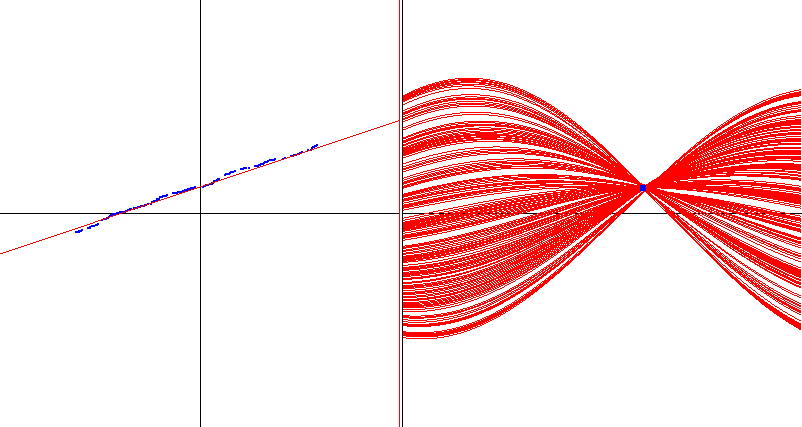
\includegraphics[width=0.80\textwidth]{img/hough.png}
\end{figure}
\subsection{La rotation}
La rotation est effectue grace a une matrice de rotation. La methode consiste a assosicie chaque pixel (i, j) a une matrice [|[|i|]; [|j|]|] puis d'utilliser la formule suivate :
\\
$A_{i,j}R_{\theta} = A'_{i,j}$ avec R = [|[|cos \theta; -sin \theta|]; [|sin \theta; cos \theta|]|] 
\\
Le resultat sera alors de la forme [|[|i'|]; [|j'|]|], il faut alors creer une image d'une (diag, diag) avec diag la diagonal de l'image source, puis assigne la couleur du pixel (i, j) au pixel (i', j').

\subsection{Decoupage de l'image}
Le decoupage de l'image s'effectue en deux etapes, la premiere est de creer deux histogrammes, l'un representant le nombre de pixel noir sur sur chaque colonne et l'autre sur chaque ligne. Puis nous allons analyser chaque histogramme separement, l'histogramme va etre parcouru, et si le contenu est plus eleve qu'un certain seuil, la case sera considerer comme du texte, des premiers blocks vont donc etre forme, une fois ces blocks formees l'algorithme est reappele mais cette fois avec le deuxieme histogramme ce qui a pour effet de redecouper les blocks et d'enlever de plus en plus de parties blanches. Le processus est appele recursivement jusqu'a ce que les blocks aient la taille d'un charactere.


\subsection{Perceptron}
Un perceptron est compose dune liste de poids, grace a un certain nombre d'entre et a une fonction dite a seuil, il va fournir une sortie grace a la formule suivante:
\\
$\sigma entree_{i}.poids_{i} > seuil$
\\
 La sortie sera 1 si l'equation est verifie, 0 sinon. Par exemple un perceptron qui peut analyser une porte OU repondra a l'entree (0, 1) par 1.
\\
Une fois le perceptrion structure il faut quil puisse apprendre, cest a dire modifier ses poids pour qu'il donne de bons resultas. Pour ce faire il faut lui passer une batterie de tests avec les resultats escomptes. On va alors evaluer le neurone avec un test et regarder si le resultat est le bon, si ce n'est pas le cas le poid va alors etre corrige selon la formule suivante: 
\\
$poid = poid + entree*(sortieVoulu - sortieReel)$.
\\
 Ces tests sont effectues jusqu'a ce que toutes les sorties soient bonnes: le perceptron a alors appris.


\subsection{Réseau de neurone}
Un neurone est tres semblant a un perceptron, au fait pret que sa sortie n'est pas binaire: il n'utilise pas une fonction a seuil mais une fonction sigmoide de la forme:
\\
$f(x) = 1 / 1 + \exp ^{k.-x}$
\\
Un reseau de neurone est compose de n couche de neurone, une couche de neurone est compose de m neurone, chaque neurone est relie avec tout les neurones de la couche precedente. Un reseau de neurone prend une liste d'entree et va fournir une liste de sortie.
\newpage
\section{Conclusion}
Et c'est ainsi que petit a petit notre ocr avance pas a pas nous pensons ne pas etre en retard et avoir meme de l'avance ! 
nous devions faire pour cette soutenance :
\begin{itemize}a
  \item Chargement et pre-traitement:
    \begin{itemize}
      \item passage au niveau de gris : FAIT !
      \item les filtres : Nous avons fait le filtre median. Nous pensons implementer un filtre de meilleur qualité que le filtre median nos recherche se tournerons donc vers le filtre moyenneur et le flou gaussien certainement
      \item binarisation : l'algorithme de binarisation semble plutot performant mais je pense que nous reverrons sont implementation qui n'est pas forcement super bien faite
    \end{itemize}
  \item Rotation OK mais nous reverrons l'algorithme pour plus de precision et de rapidite !
  \item detection de zone de texte. Nous avons un XYcut fonctionnel mais nous tendons a implementer un diagrame de voronoi ou une segmentation de Docstrum si la diffisulté est surmontable
  \item Le reseau de neurone est sur de bon rail
    \end{itemize}
    Nous pensons donc avoir rempli une bonne part du marché ! après de long effort nous nous retrouverons lors de la soutenance finale ! 
\end{itemize}

\end{document}
